\documentclass[english,submission]{programming}

\usepackage[backend=biber]{biblatex}
%\usepackage{natbib}
\addbibresource{paper.bib}

\usepackage{csquotes}
\usepackage{changepage}
\usepackage{multicol}
\usepackage{ccicons}
\usepackage[many]{tcolorbox}
\lstdefinelanguage[programming]{TeX}[AlLaTeX]{TeX}{%
  deletetexcs={title,author,bibliography},%
  deletekeywords={tabular},
  morekeywords={abstract},%
  moretexcs={chapter},%
  moretexcs=[2]{title,author,subtitle,keywords,maketitle,titlerunning,authorinfo,affiliation,authorrunning,paperdetails,acks,email},
  moretexcs=[3]{addbibresource,printbibliography,bibliography},%
}%
\lstset{%
  language={[programming]TeX},%
  keywordstyle=\firamedium,
  stringstyle=\color{RosyBrown},%
  texcsstyle=*{\color{Purple}\mdseries},%
  texcsstyle=*[2]{\color{Blue1}},%
  texcsstyle=*[3]{\color{ForestGreen}},%
  commentstyle={\color{FireBrick}},%
  escapechar=`,}
\newcommand*{\CTAN}[1]{\href{http://ctan.org/tex-archive/#1}{\nolinkurl{CTAN:#1}}}
%%

\newcounter{challengen}
\newcommand{\challenge}[1]{\subsection*{\addtocounter{challengen}{1} Challenge \#\thechallengen: #1}}

\DeclareRobustCommand{\frameworkbox}[2][gray!15]{
\begin{tcolorbox}[breakable,left=3pt,right=3pt,top=3pt,bottom=3pt,colback=#1,colframe=#1,parbox=false,
  width=\dimexpr\textwidth\relax,enlarge left by=0mm,boxsep=5pt,arc=0pt,enlarge top by=0.5em,%enlarge bottom by=0.0em,
  outer arc=0pt]\setlength{\parskip}{0.5em}\setlength{\parindent}{0em}\textbf{\sffamily Framework perspective.}\quad #2
\end{tcolorbox}}

\paperdetails{
  perspective=engineering,
  area={Programming Systems},
}

\begin{document}

% define natbib citet
\newcommand{\citet}[1]{\citeauthor*{#1}~\cite{#1}}


\title{Schema Change: Challenge Problems}

\author[a]{Jonathan Edwards}%[0000-0003-1958-7967]
\authorinfo{is TBD. Contact him at \email{jonathanmedwards@gmail.com}.}
\affiliation[a]{Independent, Boston, MA, USA}

\author[b]{Tomas Petricek}%[0000-0002-7242-2208]
\authorinfo{is TBD. Contact him at \email{tomas@tomasp.net}.}
\affiliation[b]{Charles University, Prague, Czechia}

\author[c,d]{Tijs van der Storm}%[0000-0001-8853-7934]
\authorinfo{is TBD. Contact him at \email{storm@cwi.nl}.}
\affiliation[c]{Centrum Wiskunde \&\ Informatica (CWI), Amsterdam, Netherlands}
\affiliation[d]{University of Groningen, Groningen, Netherlands}

\author[e]{Geoffrey Litt}%[0000-0003-0858-5165]
\authorinfo{is TBD. Contact him at \email{gklitt@gmail.com}.}
\affiliation[e]{Ink \& Switch, Planet Earth}

\authorrunning{J. Edwards, T. Petricek, T. van der Storm, G. Litt}

\keywords{schema change, database migration, live programming, local-first programming}

% TODO: Please go to https://dl.acm.org/ccs/ccs.cfm and generate your Classification System

\maketitle

\begin{abstract}
Schema change is an unsolved problem in both live programming and local-first software. We include
in schema change any change to the expected shape of data, whether that is expressed explicitly
in a database schema or type system, or whether those expectations are implicit in the behavior
of the code.

Schema changes during live programming can create a mismatch between the code and
data in the running environment. Correspondingly, Schema changes in local-first programming can
create mismatches between data in different replicas, and between data in a replica and the code
colocated with it. In all of these situations the problem of schema change is to migrate or
translate existing data in coordination with changes to the code.

This paper contributes a set of concrete scenarios involving schema change that are offered as
challenge problems to the live programming and local-first communities. We hope that these
problems will spur progress by providing concrete objectives and a basis for comparing alternative
solutions.

~

~


\noindent\textbf{Context}: \emph{What is the broad context of the work? What is the importance of the general research area?}
Schema change is an unsolved problem in live and local-first programming that is poorly understood and calls for a more fundamental analysis. It is particularly important as more programming
is done in programming systems where programs may be changed by their users and as more programming
is local-first, meaning that such changes need to be synchronized.

\noindent\textbf{Inquiry}: \emph{What problem or question does the paper address? How has this problem or question been addressed?}
Specific systems have specific solutions, but what is lacking is a general framework for thinking
about schema change and also a good suite of challenge problems to motivate and evaluate new solutions.

\noindent\textbf{Approach}: \emph{What was done that unveiled new knowledge?}
We collect challenge problems from a range of different kinds of (primarily) live and local-first
application contexts. We develop a framework for thinking about program change and use it to
present our challenge problems in a systematic way.

\noindent\textbf{Knowledge}: \emph{What new facts were uncovered? What new capabilities are enabled by the work?}
We understand change in programs in a novel way, using a two-dimensional framwork that looks at
the different pace layers in a program and at the different ways in which change is propagated
across program variants.

\noindent\textbf{Grounding}: \emph{What argument, feasibility proof, artifacts, or results and evaluation support this work?}
We use the framework to provide a framing for a range of challenge problems derived from both
existing literature and our own expertise.

\noindent\textbf{Importance}: \emph{Why does this work matter?}
This paper contributes a set of concrete scenarios involving schema change that are offered as
challenge problems to the live programming and local-first communities. We hope that these
problems will spur progress by providing concrete objectives and a basis for comparing alternative
solutions.

\end{abstract}

\section{Introduction}

\textcolor{red}{[JE] We should adopt the term Schema Evolution, which is favored in the research literature, defined to include schema change, data migration, and query rewriting. }

Schema change won't go away. Changing requirements and changing code lead to changing the schema of a database. Schema change, also called schema migration, is the problem of migrating existing data from the old schema to the new. This often involves custom migration programs or specialized Domain Specific Langiuages. The migration must be carefully coordinated with upgrading the application code and associated artifacts that assume the new schema. Schema change on database servers is often delegated to Database Administrators and DevOps. Live programming~\cite{tanimoto90,Hancock03} and local-first software~\cite{localfirst} both move data away from the server, eliminating those jobs, but not eliminating the need to do schema change, and indeed increasing the need to do it automatically. Recently \citet{Cambria} spotlighted these problems and proposed an approach using lenses~\cite{Foster2007}, but otherwise there has been surprisingly little research. To promote further progress we offer a set of challenge problems to the live programming and local-first communities, inviting them to propose and compare solutions.

Live programming seeks to erase the boundary between editing and running programs. In order to do so program data must be kept around while the program is being edited. Classic Lisp and Smalltalk systems integrated code and data into a persistent \textit{image}~\cite{Sandewall78, Goldberg80}. An interactive shell or \textit{Read Eval Print Loop (REPL)}~\cite{Deutsch64} is more transient than an image, but still builds up a context of data over long-lived programming sessions the loss of which disrupts the programmer's workflow. In all of these environments programs eventually get changed to create and expect data in a form incompatible with extant data. This happens whether or not the form of the data is specified explicitly in a type system or database schema, or whether it is left implicit in the behavior of the code. Some languages can tolerate a larger set of such changes, most notably Smalltalk which will automatically insert and delete members in existing instances when a class definition is changed~\cite[pp.252-272]{Goldberg80}.\footnote{Gemstone turns the Smalltalk image into a production-quality database and accordingly provides a sophisticated schema change API~\cite{Gemstone}. Schema change won't go away.} But there is still a large class of changes that create incompatibilities with existing data, whether it is inside an image, programming environment, REPL, or an external database. Some live programming environments generate data with unit tests, but that only shifts the problem of schema change to adapting those tests. One way or another, stopping everything to manually deal with schema change contradicts the goals of live programming. Schema change won't go away.

Local-first software faces related problems. Its goal is to empower users by moving code and data from the cloud to the user's own devices. Distributed programming techniques like Convergent Replicated Data Types (CRDTs)~\cite{Shapiro11} are used to coordinate data changes peer-to-peer. Unfortunately these techniques so far have not addressed schema change nor code deployment The traditional techniques of schema change used in centrally managed databases are complicated by the distributed and intermittently connected nature of local-first data. Schema change won't go away.

In the following sections we present a series of challenge problems dealing with schema change in the context of live programming and local-first software. These problems are necessarily expressed using established idioms or conventions, but nevertheless we welcome solutions that translate the spirit of the problem into other contexts.

~

~

\textcolor{red}{TODO: Need to explain that we take the programming system view - program is not something
built centrally, but something that exists and can be modified}

~

\textcolor{red}{TODO: Maybe the right way to frame this is to say that the challenges are intended
less for evaluating particular solutions but more for framing and making sense of different
kinds of schema-change-related problems.  You can read this paper and when you face a schema-change-related
problem, think about it in terms of our dimensions. Maybe compare it to our challenges.
We do not necessarilly expect that people will directly solve our challenges though. (Although
some might and that would be nice..)}

~

\textcolor{red}{TODO: I also guess this is more about just ``change'' than ``schema change''
which is one particular (most challenging) instance - i.e., change at the most permanent
pace layer.}

\newpage
\section{Dimensions of change}

\begin{figure}[t]
\vspace{-1em}
\centering
\includegraphics[width=0.5\textwidth]{figures/layers.png}
\caption{Pace layers from Stewart Brand's classic \emph{How Buildings Learn} \cite{Brand95}.
  The outer layers rarely change, while the inner layers change frequently. The geographic
  site of a building is eternal, its structure remains stable for decades, space plan
  needs to change every couple of years. ``Because of the different rates of change of its
  components, a building is always tearing itself apart.''
  \textcolor{red}{[JE] Except the outer skin changes faster than the structure.}
  }
\label{fig:layers}
\end{figure}

\textcolor{red}{[JE] `change in a program' might be misunderstood as changes to the source code. Perhaps `system' or `software system' might be better than `program'? }

In the broadest sense, this paper is concerned with the difficulties posed by a change
in a program. The first dimension of difficulties that we consider in this paper is
local. When something in a program changes, other parts of the program typically
need to be brought to sync with the changed part. The complexity of the problem varies.
If nothing else in the program depends on the changed part, for example when changing
a runtime value of an object field, the change poses no difficulty.
If many other parts of the program depend on the changed part, the difficulty is greater.
For example, if we change the schema of data structures used in the program, we also need to
change code that works with it and existing data that the users created. To structure our
discussion about this part of the problem, we will use the idea of pace layers introduced by
Brand \cite{Brand95,Brand18} (Figure~\ref{fig:layers}).

The second dimension that we consider in this paper is non-local. A program may have multiple
variants that exist independently and need to be synchronized. The difficulty of the problem
depends on what kind of synchronization we want to support. In the easier case, all variants
of the program converge, i.e.~all variants should eventually adopt all changes. In the more
challenging case, variants of a program may diverge, i.e.~a user may want to apply only certain
changes from other users. Note the non-local dimension may interact with the pace layers of the
local dimension. A typical case may be that the code and schema of a program should converge,
while data and the transient state of a program may diverge.

\paragraph{Dimensions.}
The framework for talking about schema change used in this paper thus distinguishes between
two dimensions:

\begin{itemize}
  \item The \emph{local dimension} is concerned with difficulties that a change causes
    across different program pace layers that exist within a single program.
  \item The \emph{non-local dimension} is concerned with the difficulties that a change causes
    across different program variants that exist independently.
\end{itemize}

\paragraph{Program pace layers.} As with buildings (Figure~\ref{fig:layers}), programs consist
of multiple pace layers that change at a different rate. As with buildings, making a change
to a more permanent layer also typically affects all the less permanent layers. Making a change
at a more permanent layer is thus more challenging. Alas, changing more permanent structures in
programming is frequently necessary. In this paper, we distinguish between four layers.

\begin{itemize}
\item \emph{State} -- transient state of a program. This is typically never shared across
  multiple variants of a program and it can often be discarded when a change occurs.
\item \emph{Data} -- data collected by the program. This represents a more permanent structure
  that is typically stored in a database and outlives program restarts.
\item \emph{Code} -- program logic. This layer changes whenever any aspect of the program logic
  is modified. A change typically affects transient state, but may not affect data.
\item \emph{Schema} -- the structures of program data. A change at this layer typically
  requires adapting code to work with the new structure and also updating data and state.
\end{itemize}

\paragraph{Program variants.} We are interested in programs that are distributed across multiple
environments as, for example, in local-first software. As discussed earlier, one aspect of this
dimension is whether all variants of a program eventually converge or whether it is possible to
maintain a diverging version. It is also useful to distinguish the directions in which a
change may flow, i.e., can a change originate in any variant or is there a single centralized
source of change. Note that each of this characteristics may  be associated with individual pace
layers of a program.

\begin{itemize}
\item \emph{Convergence} vs. \emph{Divergence}. In the convergence model, all program variants
  eventually adopt all changes. It may not be possible to adopt a particular change before adopting
  other changes it depends on. In the divergence model, a user may choose only particular changes
  they want to adopt.
\item \emph{Centralized} vs. \emph{Decentralized}. In the centralized model, changes (at a
  specific layer) can only originate from a particular source. In the decentralized model,
  changes can be done on any of the multiple co-existing variants of a program.
\end{itemize}

\paragraph{Challenge problems.}
The framework outlined above offers a wide range of configurations and one could conceive of
a challenge problem for many of those configurations. We can start with a change at each of the
four layers, consider each of the four configurations with respect to program variants (and also
consider different behaviour at all the affected less permanent layers). The aim of this paper
is, however, not to enumerate all options. Instead, our goal is to present a number of typical
and often encountered challenge problems. We use the above framework to more precisely define
the nature of the challenge problem. We also often use the above framework to discuss variations
on the particular challenge.

\section{Related Work}

Schema evolution has long been a major problem for SQL databases, which provide suprisingly little help. SQLite~\cite{sqliteDatatypes} uses dynamically typed values allowing them to be implicitly converted if the datatype of the column changes. MYSql~\cite{mysqlAlterTable} can reorder columns without destroying their data. But apart from such special cases, SQL databases have no general purpose support for data migration. As a result in practice schema evolution is still mostly done by writing custom SQL code to alter the schema and migrate the data. Such custom code is greatly complicated if it needs to be done without taking the database offline or must be coordinated across multiple shards. In \textit{Refactoring Databases} \citet{ambler06} offer a comprehensive taxonomy of schema evolution patterns, including typical strategies for online migration and sample SQL implementations.

\citet{bernstein07} observed in 2007 ``There are hardly any schema evolution tools today. This is rather surprising since there is a huge literature on schema evolution spanning more than two decades.'' There are now more tools available. Some tools such as Liquibase~\cite{liquibase} and PlanetScale\cite{planetscale} could be characterized as version control and continuous integration/deployment for schema. They track schema changes and can calculate diffs in the form of SQL DDL statements to convert one schema version to another, but do not help migrate data. Unfortunately comparing schemas can be ambiguous about the intention of changes. For example has a column been renamed or has it been deleted and a new one created? That distinction makes a big difference to the data in that column. EvolveDB\cite{evolvedb} addresses this ambiguity by reverse-engineering the schema into a richer data model and tracking the edits to that model within an IDE. This more precise edit history can be used to infer higher level intentions of a schema change, which then generate SQL scripts to evolve the database. EdgeDB~\cite{edgedb} resolves ambiguities by asking questions of the developer, with some answers supplying custom migration code in a proprietary query language.

Some tools provide a Domain Specific Language (DSL) to describe schema evolution. Rails Migrations~\cite{RailsMigrations} embeds a DSL in Ruby to describe a range of common schema evolutions. However that falls short of the range of evolutions described by \citet{ambler06}, requiring the addition of custom Ruby or SQL code. \citet{curino08} spawned a stream of research on Database Evolution Languages (DEL) by defining a Schema Modification Operator (SMO) as ``a function that receives as input a relational schema and the underlying database, and produces as output a (modified) version of the input schema and a migrated version of the database''. SMOs can also rewrite queries to accomodate schema changes. \citet{herrmann15} defined a relationally complete DEL and then extended it into a Bidirectional Database Evolution Language (BiDEL)~\cite{herrmann17}. BiDEL appears capable of handling the basic requirements of our Extract Entity and Multiplicity Change challenges, though Split/Merge Entity is less clear. It provides schema divergence by supporting multiple schema within one database, but would need some extension to handle data divergence.

Schema evolution is also a problem for NoSQL~\cite{sadalage12} databases. While such databases are sometimes called ``schemaless'' in effect that means the schema is left implicit and tools must try to infer it~\cite{storl20, storl22}. \citet{Cambria} uses lenses~\cite{Foster2007} for bidirectional transformation of JSON. \citet{scherzinger13} define a set of operators like the relational SMOs discussed above. \citeauthor*{chillon21}~\cite{chillon21, chillon22} offer a more comprehensive set of SMOs that may be capable of handling Extract Entity and Multiplicity Change but not Split/Merge Entity nor divergence. None of the above approaches to NoSQL evolution have yet extended into updating code or rewriting queries like their SQL cousins.

Schema evolution has also been studied for Object Oriented Databases(OODB)~\cite{li99,banerjee87}. Smalltalk~\cite{Goldberg80} is itself an OODB, persisting all object instances in an ``image file'' with some evolution capabilities incorporated in the programming environment~\cite[pp.252-272]{Goldberg80}. Gemstone turns the Smalltalk image into a production-quality database and accordingly provides a complex schema evolution API~\cite{Gemstone}.

\begin{comment}

Convex migration DSL: https://stack.convex.dev/migrating-data-with-mutations

dataframe diff https://homepages.inf.ed.ac.uk/csutton/publications/datadiff.pdf

Durable computing: pins runtime data frames to code versions. Doesn’t handle problem of global data schema change.
https://restate.dev/blog/solving-durable-executions-immutability-problem/
https://restate.dev/blog/code-that-sleeps-for-a-month/

Tijs on Live programming and model-driven engineering
https://ir.cwi.nl/pub/23770
https://dl.acm.org/doi/10.1007/s10270-017-0608-7
https://dl.acm.org/doi/10.1145/3276604.3276611
https://ir.cwi.nl/pub/21858


From Geoffrey:
1) Finding Data Compatibility Bugs with JSON Subschema Checking
https://dl.acm.org/doi/pdf/10.1145/3460319.3464796
I just found this paper this morning so I haven't read it yet, but the abstract seems very relevant. It's about automatically determining whether two JSON schemas are "compatible", with a subtyping metaphor.
2) Confluent Schema Registry:
https://docs.confluent.io/platform/current/schema-registry/index.html
An interesting example of how schema change is handled in the wild. In the Cambria essay we wrote some reflections on it which basically capture my opinions.
\end{comment}

\newpage

\section{Extract Entity}

\subsection{Context}
In this challenge we consider a typical example of how the design of a database evolves as new needs are discovered. Much has been written on the subject of data modeling methodologies and the theory of relational database normalization~\cite{Molina08}. But that work often focuses on determining the correct data model up front before the system goes live, which would indeed be the optimal solution if only we were omniscient. The Extract Entity challenge confronts the practical reality of evolving a relational data model in flight.

\subsection{Example}
The Acme Corporation needs to record orders from various customers for various products. The simplest implementation is a spreadsheet with a row for each order and columns for information about the customer and product. It might look like this:


\begin{table}[h!]
\centering
  \begin{tabular}{ |l|c|c|l|l|}
   \hline
   Item & Quantity & Ship Date & Customer name & Customer address \\
   \hline \hline
   Anvil & 1 & 2/3/23 & Wile E Coyote & 123 Desert Station \\
   \hline
   Dynamite & 2 & & Daffy Duck & White Rock Lake \\
   \hline
   Bird Seed & 1 & & Wile E Coyote & 123 Desert Station \\
   \hline
  \end{tabular}
\caption{Orders}
\end{table}

The shipping department filters this table on blank ship dates to see what they need to ship. But after a while the orders department realizes they are wasting effort duplicating the address for new order from an old customer. And when the customer's address changes they have to go back and edit all of their orders. What is needed is two tables, one with orders that links to one with customers, like this:

\begin{table}[h!]
  \centering
    \begin{tabular}{ |l|l|}
      \hline
      Name & Address \\
      \hline \hline
      Wile E Coyote & 123 Desert Station \\
      \hline
      Daffy Duck & White Rock Lake \\
      \hline
    \end{tabular}
  \caption{Customers}
\end{table}

\begin{table}[h!]
  \centering
    \begin{tabular}{ |l|c|c|l|}
     \hline
     Item & Quantity & Ship Date & Customer name \\
     \hline \hline
     Anvil & 1 & 2/3/23 & Wile E Coyote \\
     \hline
     Dynamite & 2 & & Daffy Duck  \\
     \hline
     Bird Seed & 1 & & Wile E Coyote \\
     \hline
    \end{tabular}
  \caption{Orders linking to Customers}
\end{table}

We often encounter this sort of design change when we realize that attributes of one type of entity should actually belong to a new type of entity that will be associated with the first one. Often the motivation is to centralize changes to those attributes in one place. We call this operation \textit{Extract Entity}.

In a SQL database, \texttt{Customers.Name} would be a primary key and \texttt{Orders.Customer} would be a foreign key. But before \texttt{Customers.Name} can be made a primary key the two occurrences of \texttt{Wile E Coyote} must be deduplicated one way or another~\cite{dedupe}.

\textcolor{red}{this paragraph is now redundant with Related Owrk}
Given the dominance of SQL databases it is not surprising that there are many tools for performing schema change on them~\cite{RailsMigrations, liquibase}. We do find it surprising how low-level these tools are. There is support for the basic SQL DDL commands like adding and dropping tables, columns, or constraints, but no higher level operations that would help solve our problem. One is left to write custom SQL, which can become difficult if the migration needs to be performed online without bring down the database. There is a rich theory of relational database \textit{normalization} based on \textit{functional dependencies}~\cite{Molina08} but that theory has not been implemented into schema change operations in databases -- all you get is SQL. \citet{ambler06} define higher-level patterns of schema change like \textit{Split Table} that sketch SQL implementations but don't provide everything required for Extract Entity. These difficulties fairly beg for new linguistic abstractions, though programming patterns and APIs are reasonable pragmatic solutions to our challenge.

The Extract Entity schema change is straightforward in a spreadsheet. The \texttt{Customer Name} and \texttt{Customer Address} columns are copied and pasted into a new Customers table. The \textit{Remove Duplicates} command is used to deduplicate the customers. To preserve the original view for the shipping department the \texttt{Customer Address} column is redefined with a \texttt{VLOOKUP} formula to pull the address out of the customer table based on the customer's name. A spreadsheet won't maintain referential integrity between the two tables, but end-user database tools can do that~\cite{airtable, notion}.

\subsection{Challenge}
The Extract Entity challenge for live programming is to provide interactive operations in the programming environment that will perform the schema change on live code and data. The data can be in any form desired, including relations, objects, or JSON. The code can be a simple CRUD UI that also provides the shipping department its view of unshipped orders. The central problem is to coordinate the schema change with code edits/refactorings to keep the system executing live and correctly. Solutions should try to minimize:

\begin{enumerate}
  \item The number and complexity of commands or UI affordances that must be introduced.
  \item Interruption to live execution of the code.
\end{enumerate}

The Extract Entity challenge for local-first software is similar to the live programming challenge except that the context is an application that offers similar functionality with peer-to-peer collaboration. In this context the schema change does not need to be performed interactively — a developer can take some time to build, test, and package a solution, perhaps using an API or DSL. The hard part comes when the schema change is to be deployed across all the replicas. This deployment must synchronize code and data upgrades (or decouple them as in Cambria~\cite{Cambria}). The deployment must also deal with migrating ``in flight'' operations so that all replicas converge on the same state without data loss, and ideally without centralized coordination. A radical approach could try to incorporate schema change operations into the underlying datastore/CRDT itself and integrate code as well, but layered solutions are welcome too.

\subsection{Goals}
Solutions should try to minimize:

\begin{enumerate}
  \item The need for users to manually intervene.
  \item Possibilities that developer-written code is subtly incorrect in edge cases, preferably by reducing the need for developer-written code.
  \item The need for a centralized coordinator.
  \item How long replicas might be partitioned until resynchronization is acquired.
\end{enumerate}



\section{Divergence Control}

\subsection{Context}
Schema change is usually concerned with migrating old data into a new schema. But sometimes we also want to migrate in the reverse direction: new data into an old schema. \citet{Cambria} discuss various ways that code changes can require bidirectional migration. Instead in this problem we focus on changes made by end-users. Users frequently make copies of structured documents like spreadsheets and then diverge them by altering both data content and schema. In the case of spreadsheets schema changes include rearrangements to the structure of rows and columns as well as changes to formulas. The problem is that the users want to transfer such data and schema changes between these divergent copies, and they want to pick and choose which of these changes to transfer. In practice such transfer is done manually through copy \& paste. \citet{Basman19} has documented an ecology of emailed spreadsheets. \citet{Burnett14} distilled field observations of these practices in the story of Frieda, which we quote here:

\begin{quotation}

For example, consider ``Frieda'', an office manager in charge of her department's budget tracking. (Frieda was a participant in a set of interviews with spreadsheet users that the first author conducted. Frieda is not her real name.) Every year, the company she works for produces an updated budget tracking spreadsheet with the newest reporting requirements embedded in its structure and formulas. But this spreadsheet is not a perfect fit to the kinds of projects and sub-budgets she manages, so every year Frieda needs to change it. She does this by working with four variants of the spreadsheet at once: the one the company sent out last year (we will call it Official-lastYear), the one she derived from that one to fit her department's needs (Dept-lastYear), the one the company sent out this year (Official-thisYear), and the one she is trying to put together for this year (Dept-thisYear).

Using these four variants, Frieda exploratively mixes reverse engineering, reuse, programming, testing, and debugging, mostly by trial-and-error. She begins this process by reminding herself of ways she changed last year's by reverse engineering a few of the differences between Official-lastYear and Dept-lastYear. She then looks at the same portions of Official-thisYear to see if those same changes can easily be made, given her department's current needs.

She can reuse some of these same changes this year, but copying them into Dept-thisYear is troublesome, with some of the formulas automatically adjusting themselves to refer to Dept-lastYear. She patches these up (if she notices them), then tries out some new columns or sections of Dept-thisYear to reflect her new projects. She mixes in ``testing'' along the way by entering some of the budget values for this year and eyeballing the values that come out, then debugs if she notices something amiss. At some point, she moves on to another set of related columns, repeating the cycle for these. Frieda has learned over the years to save some of her spreadsheet variants along the way (using a different filename for each), because she might decide that the way she did some of her changes was a bad idea, and she wants to revert to try a different way she had started before.
\end{quotation}

\subsection{Example}
The Divergence Control challenge instantiates the problem of divergent state with the example from the Extract Entity challenge. Every month the orders department sends its spreadsheet to the accounting department, which adds the data to a version of the spreadsheet that it has customized for financial tracking. But when the orders department migrates its spreadsheet to extract out customers the accounting department does not want to conform. They could manually convert incoming data in the new schema into their variant of the old schema. But they shouldn't have to. It should be possible to run new data through the schema change in reverse, converting it back into the format the accounting department is used to ingesting. Note that this is not a matter of synchronizing the divergent spreadsheets -- they maintain differently evolved schema.

\subsection{Challenge}
What is needed is a user-friendly mechanism for transferring data changes from one schema to another bidirectionally. In one direction we want to transfer changes made in the new schema into a variant of the old schema. The opposite direction might be needed, for example, if the accounting department makes corrections to customer addresses, which ought to be pushed through into the orders department's new schema.

Bidirectional transfer of changes between divergent copies is similar in some ways to source code version control as in Git~\cite{ProGit}. There is \textit{forking} of long-lived divergent copies. We want to \textit{diff} these forks to see exactly how they have diverged. We want to partially \textit{merge} them by \textit{cherry picking} certain differences. Yet there are also many dissimilarities with Git: our data is more richly structured than lines of text; our schema changes are higher-level transformations on these structures than inserting and deleting characters; and we expect that end-users be able to understand it~\cite{gitless}. The Divergence Control challenge is in a sense to provide ``version control for schema change'' meeting these criteria, with the key technical challenge being the ability to transfer selected differences bidirectionally through schema changes as independently as possible.

\subsection{Goals}
This challenge invites a change of perspective in both live programming and local-first software. Live programming must move from being a solitary activity to a collaborative workflow, and one where the collaboration is not just on editing source code but on live integrated code and data, as in the Smalltalk/Lisp images of old.\footnote{If only we had this in the 90's when Smalltalk had a shot at the mainstream!} For its part, local-first software must move from automatically converging data replicas to also interactively managing long-term divergence. That implies either application state is being directly exposed to the user, or the application code is using an API to present version control affordances. We encourage both communities to think outside the box of Git, which has proven to baffle not only end-users but also a substantial fraction of developers.


\newpage

\begin{figure}
\begin{adjustwidth}{-5.5em}{-5.5em}
\centering
\begin{subfigure}[b]{23em}\vspace{0pt}
   \fbox{\parbox{22.6em}{
   \textbf{PROGRAMMING CONFERENCE 2023}\\
   \textbf{Invited speakers}
   \begin{itemize}
    \item Adele Goldberg, adele@xerox.com
    \item Margaret Hamilton, hamilton@mit.com
    \item Betty Jean Jennings, betty@rand.com
   \end{itemize}
   \vspace{1em}
   }}
   \caption{Initial state of the document.}
   \label{fig:conf-orig}
\end{subfigure}
\hfill
\begin{subfigure}[b]{23em}\vspace{0pt}
   \fbox{\parbox{22.6em}{
   \textbf{PROGRAMMING CONFERENCE 2023}\\
   \textbf{Invited speakers}
   \begin{itemize}
    \item Ada Lovelace, ada@rsoc.ac.uk
    \item Adele Goldberg, adele@xerox.com
    \item Betty Jean Jennings, betty@rand.com
    \item Margaret Hamilton, hamilton@mit.com
   \end{itemize}
   }}
   \caption{Added a speaker and sorted the list.}
   \label{fig:conf-add}
\end{subfigure}
\\~\\
\begin{subfigure}[b]{23em}\vspace{0pt}
   \fbox{\parbox{22.6em}{
   \textbf{PROGRAMMING CONFERENCE 2023}\\
   \textbf{Invited speakers}

   \begin{tabular}{| l | l | l |}
     \hline
     \textbf{Name} & \textbf{Email} & \textbf{Who} \\
     \hline \hline
     Adele Goldberg & adele@xerox.com & TP\\
     \hline
     Margaret Hamilton & hamilton@mit.com & JE\\
     \hline
     Betty Jean Jennings & betty@rand.com & JE\\
     \hline
   \end{tabular}
   \\~
   }}
   \caption{Refactored list into a table.}
   \label{fig:conf-tab}
\end{subfigure}
\hfill
\begin{subfigure}[b]{23em}\vspace{0pt}
   \fbox{\parbox{22.6em}{
   \textbf{PROGRAMMING CONFERENCE 2023}\\
   \textbf{Invited speakers}

   \begin{tabular}{| l | l | l |}
     \hline
     \textbf{Name} & \textbf{Email} & \textbf{Who} \\
     \hline \hline
     Ada Lovelace & ada@rsoc.ac.uk & \\
     \hline
     Adele Goldberg & adele@xerox.com & TP\\
     \hline
     Betty Jean Jennings & betty@rand.com & JE\\
     \hline
     Margaret Hamilton & hamilton@mit.com & JE\\
     \hline
   \end{tabular}
   }}
   \caption{Resulting document after change merging.}
   \label{fig:conf-fin}
\end{subfigure}
\end{adjustwidth}
\vspace{0.5em}
\caption{Conference organizer. Initial version of the document with two independent changes
and the final version of the document after the two changes are merged.}
\label{fig:conf}
\vspace{0.5em}
\end{figure}


\section{Conference Organizer: Merging edits in computational documents}
In this section, we consider challenges related to working with a document-based format akin to HTML.
We discuss two variants of the format. In the first format, a document
contains only data. In the second variant, the format is extended with computed values.
A computed value is a node in the document whose value is specified by a formula akin to those
used in spreadsheets. The equations can refer to other nodes in the document, possibly using
an absolute or a relative path and may involve a range of built-in functions, for example to
count the number of elements or to sum a sequence of numerical values.

We assume that the document can be
concurrently edited by multiple users in the same fashion as in local-first software, i.e.,
users may edit a local copy that then needs to be synchronized with changes made by other users.
The edits to the document can be done in a rich-text editor, or by using a more structure-aware
structure editor that can, for example, record changes as a sequence of high-level edit operations.

The concrete challenges are centered around the problem of collaborative conference planning
as illustrated in Figure~\ref{fig:conf}. A number of co-organizers are planning a conference
that will feature talks by several invited speakers. They need to agree on the speaker list,
contact speakers and calculate the conference budget.


\frameworkbox{
In this scenario, the only transient \emph{state} is the result of computed values. The content
of the document corresponds to the \emph{data} pace layer. A change in the data layer may invalidate
the computed value at the state layer. Formulas correspond to the \emph{code} layer and changing them,
again, invalidates the state. The \emph{schema} pace layer is implicit. A change to the document that
modifies content is a mere data change, but restructuring the document is an implicit schema
change. Such schema change that may affect the code pace layer.

The scenario assumes the \emph{decentralized} model. There are multiple program (document)
variants and it should be possible to propagate a change at any pace layer to other program
variants. The challenge may be solved using both the easier \emph{convergence} and the more
challenging \emph{divergence} model.}

\paragraph{Applications.}
One of the earliest systems to combine documents with computational elements
is Boxer \cite{diSessa86}. The challenges in this section apply to a wide range of
systems that can be seen as its successors. The specific scenario discussed here is
inspired by the use of Notion~\cite{notion}, which is a collaborative structured document
editing system. Treating documents as end-user programs has recently
been explored in Potluck~\cite{Litt2023}, which is local-only but includes formulas similar
to those in our challenge.

The challenges in this section are also relevant to work on computational scientific notebooks.
Jupyter \cite{Kluyver2016} uses a simple representation as a sequence of cells and does not have
a mechanism for embedding data in the document and referring to it, but numerous
project such as Nextjournal \cite{Nextjournal21} advance the format. The idea of producing
interactive, computational secientific documents is an active research area. Recent contributions
include Nota~\cite{Crichton2021} and Living Papers \cite{Heer2023}.

\challenge{Merging structured document edits}

First, the organizers need to agree on a list of speakers to invite, coordinate who contacts
whom and track the acceptance of invitations. They start with a document shown in
Figure~\ref{fig:conf-orig}. The challenge is to merge document edits that are done locally
and independently by two co-organizers. Specifically, consider the following two edits:

\begin{enumerate}
\item The first organizer adds an additional speaker to the list and sorts the list of speakers
  alphabetically by their first name. (Figure~\ref{fig:conf-add})
\item The second organizer refactors the list into a table. They split the single textual value
  into a name and an email (using a comma as the separator) and add an additional column for
  tracking which of the organizers should contact the speaker.
\end{enumerate}

\noindent
The system should be able to merge the changes and produce a final table shown in
Figure~\ref{fig:conf-fin}. The resulting table needs to include the additional speaker
created by the first organizer, use the order specified by the first organizer and use
the format defined by the second organizer. The newly added speaker should be reformatted
into the new format. For the newly added ``Organizer'' column, the second user may
specify default value or the newly added row may use an empty value.

\frameworkbox{
In this challenge, the change done by the first organizer is at the \emph{data} layer,
while the change done by the second organizer spans the \emph{schema} and \emph{data} layers.
In implementing the schema change, the second organizer transforms the affected document data.
The challenge is to apply the same transformation to the data independently added by the
second organizer.
}

\paragraph{Requirements.}
The challenge is concerned with merging two sequences edits to a base document.
A solution to the challenge should strive to satisfy the following goals:

\begin{itemize}
\item \emph{Completeness.} It should be possible to semi-automatically merge any two sequences
  of edits. In other words, the merging should always be defined, regardless of what edits the
  users perform, although user input may sometimes be necessary.
\item \emph{Commutativity.} The order of edits should not matter, regardless of their pace layer.
  If users $A$ and $B$ perform edits independently starting from the same initial document, the
  resulting document should be the same if the system treats edits from $A$ as occurring before
  the edits of $B$ and vice versa.
\item \emph{Conflict resolution.} It may not always be possible to merge conflicting edits.
  In this case, the system should interactively ask the user for guidance or, possibly, use
  default behavior specified by the user.
\item \emph{Structure editing.} The system may use a structure editor that provides high-level
  commands for operations such as reordering of elements or refactoring of a list into a table.
  In other words, we recognise that the challenge may not be solvable in a system based on plain
  text editing of document source code.
\end{itemize}

\paragraph{Remarks.}
As discussed earlier, this challenge does not make an explicit distinction between the schema
of the document and data. The implementing system may or may not maintain such distinction.
In our example, adding a new speaker and sorting the list is a mere change of the data, but the
refactoring of a list into a table is a schema change. The system may offer different user interface
for changes at different layers and leverage knowledge about such distinction, for example,
by handling the merging of schema-related and data-related changes differently.


\begin{figure}
\begin{adjustwidth}{-5.5em}{-5.5em}
\centering
\begin{subfigure}[b]{23em}\vspace{0pt}
   \fbox{\parbox{22.6em}{
   \textbf{PROGRAMMING CONFERENCE 2023}\\
   \textbf{Invited speakers}
   \begin{itemize}
    \item Adele Goldberg, adele@xerox.com
    \item Margaret Hamilton, hamilton@mit.com
    \item Betty Jean Jennings, betty@rand.com
   \end{itemize}
   \vspace{1.5em}
   \textbf{Conference budget}\\
   Travel cost per speaker:\\
   \hspace*{2em} \$1200 \\
   Number of speakers: \\
   \hspace*{2em} \texttt{=COUNT(/ul[id='speakers']/li)} \\
   Travel expenses:\\
   \hspace*{2em} \texttt{=/dl/dd[0] * /dl/dd[1]}
   }}
   \caption{Initial state of the document with formulas.}
   \label{fig:conf-budget}
\end{subfigure}
\hfill
\begin{subfigure}[b]{23em}\vspace{0pt}
   \fbox{\parbox{22.6em}{
   \textbf{PROGRAMMING CONFERENCE 2023}\\
   \textbf{Invited speakers}

   \begin{tabular}{| l | l | l |}
     \hline
     \textbf{Name} & \textbf{Email} & \textbf{Who} \\
     \hline \hline
     Ada Lovelace & ada@rsoc.ac.uk & \\
     \hline
     Adele Goldberg & adele@xerox.com & TP\\
     \hline
     Betty Jean Jennings & betty@rand.com & JE\\
     \hline
     Margaret Hamilton & hamilton@mit.com & JE\\
     \hline
   \end{tabular}

   \vspace{0.5em}
   \textbf{Conference budget}\\
   Travel cost per speaker:\\
   \hspace*{2em} \$1200 \\
   Number of speakers: \\
   \hspace*{2em} \texttt{=COUNT(/table[id='speakers']/tbody/tr)} \\
   Travel expenses:\\
   \hspace*{2em} \texttt{=/dl/dd[0] * /dl/dd[1]}
   }}\caption{Resulting document after schema change merging.}
   \label{fig:conf-finfin}
\end{subfigure}
\caption{Conference organizer. Formulas to calculate the budget have been added to the
original document (Figure~\ref{fig:conf-orig}) and those have to be merged with the
refactoring of a list into a table (Fig~\ref{fig:conf-tab}). Formulas in the final version
are updated to match with the new document structure.}
\label{fig:conf-calc}
\end{adjustwidth}
\end{figure}


\challenge{Applying schema edits in presence of code}

This challenge extends the previous problem. The conference organizers now also want to use
the document to manage the conference budget. In a very simplified form, one aspect
of this is calculating the estimated travel expenses for the speakers. For this,
they add a computed value to the document that counts the number of speakers
and multiplies the result by a fixed cost per speaker elsewhere in the document.

The scenario is shown in Figure~\ref{fig:conf-budget}. Assume two co-organizers start with
the same original document shown in Figure~\ref{fig:conf-orig}. One adds an additional
section with computed values, while the other performs the edits discussed earlier.
The challenge is, again, to merge the edits done independently by the co-organizers.

\begin{enumerate}
\item The first co-organizer adds the budget calculation as shown in Figure~\ref{fig:conf-budget}.
  This includes two formulas. The first selects all \texttt{li} elements of a \texttt{ul} element
  with ID \texttt{speakers} (not visible in the UI) and counts their number. The second formula
  multiplies the constant travel cost per speaker by the number of speakers. Here, we assume the
  new section uses the HTML definition list \texttt{dl} and the formula selects its first and
  second \texttt{dd} item, respectively.

\item The second co-organizer performs the refactoring and data edits discussed previously.
  They edit the speakers and refactor the structure to use a table, resulting in the document
  shown in Figure~\ref{fig:conf-fin}.
\end{enumerate}

\noindent
As before, the system should be able to merge the edits made to the document.

\frameworkbox{
In this challenge, the change done by the first organizer is at the \emph{code} layer, while
the change done by the second organizer is both at the \emph{data} layer and, implicitly,
at the \emph{schema} layer. A change solely at the \emph{data} layer would not affect code,
but a change at the \emph{schema} layer requires adapting some aspects of the code.
}

\paragraph{Remarks.}
Addressing the challenge requires that the refactoring of the document structure done in (1),
is also reflected in the code of the equations added in (2). As shown in
Figure~\ref{fig:conf-finfin}, in this specific case, the system needs to change the equation
\texttt{COUNT(/ul[id='speakers']/li)} to \texttt{COUNT(/table[id='speakers']/tbody/tr)}.
This is the case because the refactoring consists of four steps that each transform the
document and also need to update the code of the equation accordingly:

\begin{itemize}
    \item[--] Change the type of the \texttt{ul} element to \texttt{table}
    \item[--] Wrap the body of the \texttt{table} element with \texttt{tbody}
    \item[--] Change the type of all children of \texttt{tbody} from \texttt{li} to \texttt{tr}
    \item[--] Further split the body into two \texttt{td} elements
\end{itemize}

\noindent
It is expected that the system solving the challenge will need to be aware of those high-level
edits. In particular, they may be explicitly specified by the user (through an interactive
user interface for editing the document) or semi-automatically inferred.

\paragraph{Requirements.}
A solution to the challenge should meet the goals of the preceding challenge, i.e., completeness
(merging should be always defined), commutativity (order does not matter), conflict resolution
(ask for guidance if needed), convergence (everyone eventually wants the same document) and
structure editing (the system may capture high-level edits).

\subsection*{Challenge Extensions: Liveness and divergence}
So far, we assumed that the system follows the \emph{convergence} model, i.e., all variants
of the program eventually adopt all changes. A more difficult variant on the challenge is to also
support the \emph{divergence} model. In this case, some of the users continue using their variant
of the program without adopting all of the changes done by other users.

\frameworkbox{
In the \emph{divergence} model, it may be expected that users will want to adopt all changes
done at the \emph{data} pace layer. They may selectively choose some of the changes at the
\emph{code} and \emph{schema} layers. The challenge is maintaining the same data across multiple
program variants and merging changes done to the data based on different document schema.
}

The basic challenge outlined above focuses primarily on the local-first software scenario, but
it can be extended to also apply to the live programming scenario. In particular, when the
document contains computed values, those may be evaluated either explicitly by the user or
automatically on-the-fly. An edit can then invalidate some of the values (either by changing
the data that a computed value depends on, or by changing the equation used to compute the value).
A live programming system should be able to detect which computed values are affected by an edit
and, either invalidate those (requiring an explicit re-evaluation by the user) or automatically
re-evaluate them (and possibly highlight the affected values to inform the user).

\frameworkbox{
In the live extension, we also consider the transient \emph{state} pace layer. A system should
automatically detect when a change at the \emph{data} or \emph{code} layers affects the computed
value and forces it to be recomputed. Interestingly, a change at the \emph{schema} layer may not
always affect the \emph{state} layer, even if it schema change requires modifying formulas that
compute the state.
}


\newpage

\section{Live Modeling Languages Require Run-Time State Migration}
%Related work
%``Slogan'': editing a program is diverging from run-time schema.

\subsection{Context}
In stateful live programming, a change in the program can make the run-time state of the execution out of date, hence we want to migrate the run-time state to keep on running.

One can see a program itself as an instance of a static schema (its AST type), that in turn determines (defines/implies/induces) a run-time schema: the run-time structures of code (e.g., classes, inheritance links, declarations, method definitions etc.), as well as the structure of the run-time state. Whereas the run-time \textit{code} structures do not typically change while using an application, the run-time \textit{state} constantly changes.
Live programming, however, requires reconciling changes to the program with the run-time structures of both the code and the state. This typically means that at a certain point (a quiescent point) during execution, the code structures need to be updated (hot swapped), and the state needs to be \textit{migrated}.

\subsection{Example}
Consider the example of a simple state machine language with on-entry actions, and typed global variables (loosely inspired by the SML language of \citet{vanRozen19}). An example state machine and an excerpt of its abstract syntax schema is shown in Figure~\ref{LST:statemachines}. Depicted on the left, an actual statemachine modeling the opening and closing of a door, with one global boolean variable, \lstinline{isClosed}, which is flipped according to transitioning between the \lstinline{closed} and \lstinline{opened} states. For the sake of brevity, the abstract syntax schema (similar, to e.g., and Ecore metamodel~\cite{EMF}) shown on the right of the figure omits classes for the on-entry actions (\lstinline{Stmt}) and variable types (\lstinline{Type}).

\begin{figure}[t]
\centering
\begin{minipage}[t]{0.4\textwidth}
\begin{lstlisting}[language=java,morekeywords={machine,on,state,var}]
machine Doors

var isClosed: bool = true

state closed
  isClosed := true
  on open => opened

state opened
  isClosed := false
  on close => closed
\end{lstlisting}
\end{minipage}
\hspace*{2pt}\vline
\begin{minipage}[t]{0.4\textwidth}
\begin{lstlisting}[language=java,morekeywords={on}]
  class Machine
    name: string
    states: State*
    vars: Decl*

  class State
    name: string
    onEntry: Stmt*
    transitions: Trans*

  class Trans
    event: string
    target: State

  class Decl
    name: string
    type: Type
  \end{lstlisting}
\end{minipage}
\caption{A statemachine and its abstract syntax schema (omitting \lstinline{Stmt} and \lstinline{Type})}
\label{LST:statemachines}
\end{figure}

In the following we assume that the state machine is executed by an interpreter that process an incoming stream of events, and traversing run-time pointers representing transitions accordingly, executing on-entry actions, where the notion of the current state and the values of the global variables are the collective run-time state of the program. The structure that the interpreter operates on can be described as derived  schema from the abstract syntax scheme shown on the right of Figure~\ref{LST:statemachines}, but specialized for a particular machine, e.g., \lstinline{Doors}.
This schema will have additional fields and associations modeling the run-time data required for execution. For the \lstinline{Doors} statemachine, this means adding the current state to the \lstinline{Machine} type (required for any machine) and the machine specific data fields, namely \lstinline{isClosed}. The run-time schema for \lstinline{Doors} is then the following\footnote{It is possible to represent the global variables at run-time using an untyped table or hashmap, but for the sake of schema migration complexity, the encoding as fields in classes is more instructive.}:
\begin{quote}
\begin{lstlisting}[language=java,morekeywords={on},mathescape=true]
class Machine$^{++}$
  states: State*
  current: State
  isClosed: bool
\end{lstlisting}
\end{quote}
This \textit{extended} class $\text{\lstinline{Machine}}^{++}$ also represents state machines, but this time at run time.



\begin{figure}[t]
  \centering
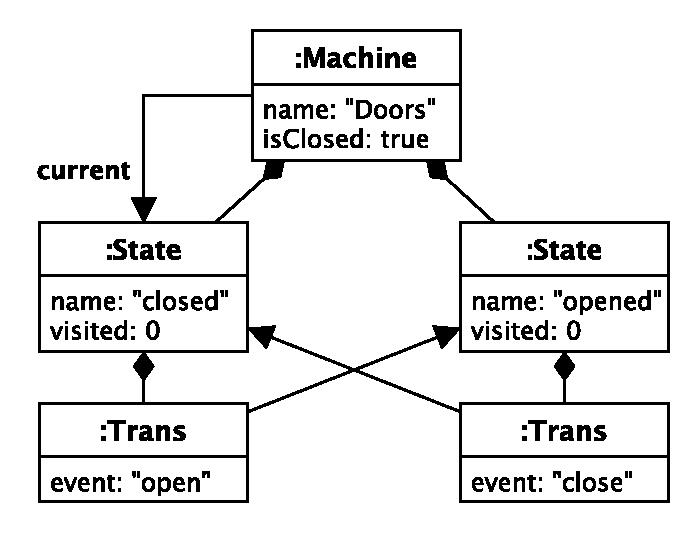
\includegraphics[width=0.5\textwidth]{figures/doorsmachine.pdf}
\caption{UML object diagram of the run-time structures of the Doors statemachine (excluding code objects)}
\label{FIG:doorsRuntime}
\end{figure}


An instance of a running state machine consists of an object graph conforming to the run-time schema of state machines, updating the \lstinline{current} state pointer in response to events. This object graph is graphically depicted in Figure~\ref{FIG:doorsRuntime} as a UML object diagram, excluding the statement objects representing on-entry actions. As the diagram shows, the running machine has a current state (\lstinline{closed}) and the \lstinline{isClosed} field has an actual value (\lstinline{true}). It is instructive to note that the diagram encode both static and dynamic aspects of the state machine language. Live editing the state machine then requires to \textit{patch}~\cite{SemanticDeltas} this run-time structure without shutting it down, possibly requiring migration of run-time state.

\subsection{Challenge}

\begin{table}[t]
  \centering
\begin{tabular}{lll}\toprule
\textsc{Change} & \textsc{What} & \textsc{How}\\\midrule
add & state & simple  \\
remove & state & structurally simple, but heuristic if state is current \\
rename & state & simple\\
add & variable & migrate class and initialize field \\
remove & variable & migrate class (NB: assumes variable is unused)\\
rename & variable & rename in class, preserving value\\
type change & variable & migrate class and convert or reinitialize value \\
add & transition & simple \\
remove & transition & structurally simple, but heuristic for pending events\\
event change & transition & structurally simple, but heuristic for pending events\\
add/remove & statement & hotswap code at quiescent point of interpreter\\
\bottomrule
\end{tabular}
\caption{Possible program changes and how to deal with them at run time}
\label{TBL:changes}
\end{table}

The space of possible (well-formed\footnote{The abstract syntax schema is not expressive enough to define all static invariants of the language, such as: states must by unique by name, references variables in actions must be declared, etc.}) changes to a state machine are summarized in Table~\ref{TBL:changes}.
The first column indicates the change category, the second the affected kind of object, and third a short description of how to deal with the respective change category. Some notes about this table:
\begin{itemize}
\item all rows with ``simple'' in the third column only require a quiescent~\cite{Tranquility} point in the interpreter loop to update the run-time structure (e.g., as shown in Figure~\ref{FIG:doorsRuntime}).
\item removing a state, however, is only \textit{structurally} simple, since removal is easy, but special care needs is required if the subject of removal is the current state. In this case, some heuristic is needed, such as: reject the edit, point the current state to the initial state, or some other strategy (e.g., the nearest state, previous state etc.)
\item everywhere a row mentions ``migrate class'' in the third column, data migration is needed: the run-time objects conforming to the old class must be transformed to instances of the updated class, similar to how Smalltalk migrates objects using \lstinline{become:}.
\item removing a transition or changing the event of a transition potentially has to deal with pending events (e.g., in an event queue) expecting such transitions, since such events are now potentially stale. Strategies to deal with this situation include: simply dropping the events, or requiring that such edits cannot be patched at run time when there are pending events.
\item the type change edit of variable requires a strategy for the current value: either discard and reinitialize, or perform value conversion. For instance, if the type change is from boolean to integer, then true could become 1, and false could become 0.
\item note finally that rename variable is mentioned explicitly as a change: this makes it possible to preserve the run-time value of the variable.
\end{itemize}

\subsection{Goals}

The goals for this challenge are twofold: from the end-user perspective and from the language engineering perspective. A particular challenge from the end-user perspective is to ``do minimal harm'': it is essential for fluid programming experience that the automatically triggered migrations are in a sense as near as possible to the previous application state, to not surprise or confuse the user/developer.
One approach  considered in earlier work~\cite{RuntimeConstraint} employs the constraint solver Z3 to find a ``nearest'' run-time instance compatible with a source change. Nevertheless, the patching of the run-time state should be quick enough so as to not disrupt the programmer experience.

From the language engineering perspective the goal is to employ techniques, formalisms, and tools, to make the construction of such languages easier. The above example state machine DSL is derived from earlier work~\cite{vanRozen19}, where the authors manually implemented the run-time patch operation and concluded that even for such a simple language (simpler even than the example above) it is a complex and error-pone endeavor. Furthermore, the field of software language engineering studies and develops generic and reusable techniques to improve the development of DSLs and programming languages, for instance, in the context of language workbenches~\cite{ERDWEG201524}. The development of live programming languages, however, is currently still out of reach for all existing language workbenches. The aforementioned approach using a constraint solver is an example of such a \textit{language parametric} technique, in that it operates on the (extended) abstract syntax metamodel of a language, and does not assume anything further about the language itself. Another approach is the \textsc{Cascade} metamodeling formalism which has builtin support for run-time patching~\cite{Cascade}. However, further research is needed to design better principled language engineering approaches that solve the problem in a way that is both declarative and fast.

\subsection{Extensions}

While the above example is arguably simple, the problem becomes much more challenging when the programs themselves define data types, classes, records, structures etc. Since possibly many instances (values, objects) of such data types may exist at run-time, these all have to be migrated in such a way that programmer experience is minimally disrupted, and that the invariants of said data types is maintained.
Another extension, tying in with the data-oriented examples above, involves refactorings of data types in a program. Typically a refactoring should be behavior preserving, but can it also preserve run-time data? The minimal example is the consistent variable rename rename in Table~\ref{TBL:changes}, which should not have any effect on run-time state.  A more complex refactoring is described in Section~\ref{SECT:elm}.

\section{Live programming in the context of Elm architecture}
\label{SECT:elm}
\subsection{Context}
Another challenge involving stateful live programming can be drawn from the programming model based on the Elm architecture. In this model, a reactive (web) application is structured in terms of current state and events that affect the state. The implementation then consists of two functions that we may call \texttt{update} and \texttt{render}:

\begin{quote}
\begin{lstlisting}[language=ml,morekeywords={on}]
type State = { .. }
type Event = .. | ..

val update : State -> Event -> State
val render : State -> Html
\end{lstlisting}
\end{quote}

The programming model works as follows:
\begin{itemize}
    \item \texttt{State} represents the entire application state, i.e., everything that the user can work with.
    \item \texttt{Event} represents all events that the user can trigger by interacting with the application.
    \item \texttt{update} is called whenever an event happens. It takes the current state, the event and computes a new state.
    \item \texttt{render} takes the current state and produces a representation of what should be displayed on the screen (e.g., an HTML tree).
\end{itemize}

Traditionally, when Elm applications are developed, they are restarted each time the code is modified and any previous state is discarded. However, a more effective programming model based on live programming would allow live updates to both the code of the two functions and the structure of the two types.

\subsection{Example}

As an example, consider the uninspiring, but well-known, TODO list application. The types that capture the state and events in the application may look as follows:

\begin{quote}
\begin{lstlisting}[language=ml,morekeywords={on}]
type Item = { id : id; title : string; completed : bool }
type State = { items : Item list }
type Event =
  | SetCompleted of id * bool
  | SetTitle of id * string
  | Remove of id
  | Add of string
\end{lstlisting}
\end{quote}

The application state consists of a list of items. Each item has a unique ID alongside with a title and a flag indicating whether it is completed. The events represent edits to the items, deletion and addition. The implementation of the \texttt{update} and \texttt{render} functions is simple and not important for the challenge.

\subsection{Challenge}
Now, imagine that we have a running TODO list application with the above state and events. To test the application, the programmer has already created a number of items and so there is a single value of the \texttt{State} type that represents a current state of the application such as:

\begin{quote}
\begin{lstlisting}[language=ml,morekeywords={on}]
{ items : [
   [ { id = 1; title = "check twitter"; completed = true  }
     { id = 1; title = "Write paper"; completed = false } ] }
\end{lstlisting}
\end{quote}

As above, there are a number of edits to the code and types that the programmer may want to do without restarting the application. Those are summarized in Table~\ref{TBL:elmchanges}. Modifying the code is simple and only requires waiting until the current execution completes. Modifying the \texttt{Event} type is also simple, but it may lead to unused code or missing case in \texttt{update} that needs to be addressed. Finally, modifying \texttt{State} ranges from relatively simple problems (adding a new field) to challenging case when the structure of \texttt{State} is changed.

For example, imagine that the programmer would want to edit the structure of the state and migrate the previous definition of \texttt{State} to the following new definition where individual fields are stored in separate lists:

\begin{quote}
\begin{lstlisting}[language=ml,morekeywords={on}]
type State =
  { ids : id list
    titles string list
    completes : bool list }
\end{lstlisting}
\end{quote}

This representation is semantically equivalent (assuming the lists have the same length) to the original one. It should thus, in principle, be possible to migrate the original state value to a value using the new structure. Moreover, it should, in principle, be also possible to automatically transform the implementations of \texttt{update} and \texttt{render} to work as before, but using the new state structure.

\begin{table}[t]
  \centering
\begin{tabular}{lll}\toprule
\textsc{Change} & \textsc{What} & \textsc{How}\\\midrule
modify & \texttt{render} & simple, but wait until current execution finishes  \\
modify & \texttt{update} & simple, but wait until current execution finishes  \\
add & case to \texttt{Event} & requires adding corresponding case to \texttt{update} \\
remove & case from \texttt{Event} & remove unused code from \texttt{update} \\
add & field to \texttt{State} & migrate state value and initialize field \\
remove & field from \texttt{State} & migrate state (assuming field unused) \\
modify & structure of \texttt{State} & migrate state value and edit code accordingly \\
\bottomrule
\end{tabular}
\caption{Possible program changes and how to deal with them at run time}
\label{TBL:elmchanges}
\end{table}


\subsection{Goals}
As above, the key requirement from the live programming perspective is to “do minimal harm”. In this case, this results in the following goals:

\begin{itemize}
\item When migrating the application state, this needs to be done automatically and the system should strive to produce new state that is as near as possible to the previous state.
\item The solution may rely on structure editing so that the system has access to a high-level logical description of the edits performed by the user.
\item The system needs to handle the case when the type structure diverges from the code structure. This can be addressed in various ways (transform code, add error handlers, etc.) but it is desirable to avoid "breaking" the \texttt{render} function as this would make the new application state impossible to see.
\end{itemize}

\subsection{Remarks}
It is worth noting that the particularly difficult aspect of this challenge, i.e., the case where the structure of state is refactored to an equivalent one, is related to the Extract Entity challenge.

\section{Multiplicity change}

\subsection{Context}

A common kind of schema change is \textit{multiplicity change}: when a field changes from storing a single value to storing multiple values. For example, we might start by storing a single address for each contact in an address book, before realizing that we need to store multiple addresses for a single contact; or we might assign each todo in a list to one person before realizing we want the ability to assign a todo to multiple people.

In a relational schema, solving this problem might require extracting a normalized table for the linked entity; some of the challenges of this approach are covered in the Extract Entity challenge. In this section we will instead consider a document schema with support for arrays; in this context, we can have a multiplicity change by turning a scalar value into an array value.

Multiplicity change clearly requires changing both the data and the code. It becomes particularly challenging to handle when there is a need to support ongoing writes to both the scalar and array schemas. This need can arise in any situation where the code and data can't all be updated atomically together—e.g., in a zero-downtime upgrade in a web architecture with stateless servers and a database, or in a decentralized setting like a public API where some consumers of the API may be expecting an outdated schema.

\subsection{Example}

Consider the following schema for a todo list item, in which each item has a single assignee, represented by a user ID:

\begin{quote}
\begin{lstlisting}[language=ml]
type Item = { id : id; title : string; assignee : string }
\end{lstlisting}
\end{quote}

Now, we change the schema so that each item has a list of assignees:

\begin{quote}
\begin{lstlisting}[language=ml]
type Item = { id : id; title : string; assignees : Array<string> }
\end{lstlisting}
\end{quote}

Our goal is to preserve the ability for actors in the system to read and write to a shared todo list in either the old or new schema—for example, they should be able to write to either the scalar assignee field or to the list of assignees.

A natural invariant to preserve across these schemas is that the value of the scalar field should equal the first element of the list field (and if the list is empty, the scalar field should be null). If we were to write code for a one-time data migration from the scalar to list schema, we could easily satisfy this invariant:

\begin{quote}
\begin{lstlisting}[language=ml]
item.assignees = if (item.assignee == null) then [] else [item.assignee]
\end{lstlisting}
\end{quote}

Ongoing edits to the array schema can also be handled in a straightforward way. After edits are made, the value of the scalar field should be set to the first element of the new array (or null if the new array is empty.)

However, handling edits to the scalar schema presents more of a challenge. Consider the following todo with two assignees, presented in terms of the scalar and array schemas. A write is made in the scalar schema to set the new assignee to C.

\begin{quote}
\begin{lstlisting}[language=ml]
todoScalar = { id: 1, title: "Foo", assignee: A }
todoArray = { id: 1, title: "Foo", assignees: [A, B] }

todoScalar.assignee = C
\end{lstlisting}
\end{quote}

What should the array value become after this edit to the scalar schema? To satisfy our invariant, we know that C must become the first element of the array, but this leaves open several options with different tradeoffs:

\begin{enumerate}
  \item \texttt{[C]}: "Only C should be assigned." This option produces an array that corresponds directly to the resulting scalar. But it has the downside of deleting data that wasn't even visible in the scalar schema.
  \item \texttt{[C, B]}: "Replace A with C." If the writer wanted to remove A from the assignment and add C, this option performs that intent. However, there is data remaining in the list which was not visible to the scalar writer.
  \item \texttt{[C, A, B]}: "Add C to the list." Perhaps the scalar writer wanted to add C to the assignment without removing anyone; this option satisfies that intent. But it preserves data not visible to the scalar schema.
\end{enumerate}

Because the intent of the writer to the scalar schema cannot be unambiguously interpreted from the write alone, it is impossible to make a perfect choice among these options.

\subsection{Challenge}

Multiplicity change illustrates a general problem for handling ongoing writes between diverging schemas. Different schemas may expose partial information, and writers in those schemas have to operate without total knowledge of the information available in other schemas. As a result, synchronizing writes across the schemas requires making difficult tradeoffs, such as choosing to either preserve or destroy hidden data not visible to the writer.

Although we see no silver bullet to navigate these tradeoffs, a good solution to this problem would give developers or users tools to manage these tradeoffs. For example, a system might allow developers to specify the desired behavior for a particular pair of schemas based on the requirements of the domain. Or a system might even allow users to manually disambiguate their intent for a given write.

\subsection{Goals}

TODO

\begin{comment}
\section{Rename field; Add new required field}
Starter problems suggested by Geoffrey. These are already directly supported in SQL, so there is good support in SQL schema change tools, but they don't address how to synchronize the change with live code refactoring or local-first code deployment.
\end{comment}

\begin{comment}
\section{Cambria (Geoffrey/pvh)}
\citet{Cambria} exhumed and studied the old problem of schema change, primarily in the context of local-first software. In this paper we add more scenarios and the complementary problems of live programming. The primary goal of local-first software is user autonomy, which could include letting users stay on older versions of application code while continuing to collaborate with newer versions. This problem is a nice counterpart to that of Divergence Control. They both require a kind of bidirectional schema change, with Cambria building upon research on bidirectional programming with lenses, while Divergence Control is more closely connected to version control techniques. Appendix III of \cite{Cambria} discusses the tricky problem of converting between scalars and arrays (which in data modeling is called a multiplicity change). That could be the challenge problem right there.

The Cambria paper also presents motivating examples of schema change problems in Stripe, Kafka, and Mastodon. Perhaps one of those examples could be crafted into a challenge problem.
\end{comment}

\begin{comment}
\section{Denormalization (Matt Tantaman)}
Matt points out Extract Entity is a normalization so we ought to complement it with a denormalization. Note that copying/duplication is a technical problem in some formalisms like lenses. Denormalization is often done for performance reasons but that isn't an issue in our small-scale scenarios. What is a small-scale use case for denormalization?

There are good cases for denormalizing from 1NF, i.e. nesting structures. Local-first software seems focused on JSON data rather than relational. An extension of Extract Entity is \textit{Nest Entity} where a table of orders are nested inside each customer.
\end{comment}

%\bibliographystyle{abbrv}
%\bibliography{paper}
\printbibliography

\end{document}

% Local Variables:
% TeX-engine: luatex
% End:
